\documentclass{article}
\usepackage[backend=biber, style=authoryear-icomp]{biblatex}
\usepackage{blindtext}
\usepackage{multicol}
\usepackage[document]{ragged2e}
\usepackage[pass, letterpaper]{geometry}
\usepackage{amsmath}
\usepackage{amsfonts}
\usepackage{xcolor}
\usepackage{caption}
\usepackage{graphicx}
\usepackage{subcaption}
\addbibresource{ref.bib}

% Define macros
\newcommand\note[1]{\textbf{\textcolor{red}{#1}}}
\newcommand{\comment}[1]{}

% Captions
\captionsetup{justification = raggedright, singlelinecheck = false, labelfont=bf}
% To cite, use \parencite{} or \textcite{}

\title{Using an Autoencoder Model to Characterize Air Pollution}
\author{Nicolas Shannon$^{1}$, Vandana Nunna Lakshmi$^{2}$}
\date{}

\begin{document}

% Indentation
\setlength{\parindent}{3ex}
\setlength{\parskip}{0.25ex}

% Acknowledgements
\begin{centering}
\maketitle
\vspace{-0.50cm}
\scriptsize
{$^{1}$Department of Computer Science, Loyola University Chicago, Chicago, IL, US}\\
{$^{2}$Department of Computer Science, University North Texas, Denton, TX, US}\\
\end{centering}

\begin{abstract}
Climate change is one of the most complex challenges humanity has ever faced. It is a
multi-dimensional problem that poses economic, social, scientific, political, and 
moral questions that must be addressed. One of the most important ways of 
combating climate change is to research pollution mitigation strategies 
so that policy makers and government planners are better equipped to  make 
informed decisions. We focused on the principle cause of global warming:
the polluting gases responsible for the rapid shift in global climate.
We characterize cities by the amount of pollution present using an undercomplete autoencoder
model. By representing the level of eight toxic gases present in numerous cities
across the United States, we explore some of the more prominent features 
that characterize urban pollution. We compare two techniques for reducing 
the dimensionality of our input - Principle Component Analysis (PCA) and
Autoencoders. The first two hidden dimensions represented
a large percentage of the explained variance in the model, so we cluster
the cities in an effort to extract any useful features. 
\end{abstract}
\vspace{0.25cm}
\section{Introduction}

\par Over the past several decades, air pollution has been a major concern for human health
and the environment. The EPA sets national air quality standards for  six major air
toxins: ground level Ozone (O$_3$), Carbon Monoxide (CO), Sulfur Dioxide (SO$_2$),
Lead (Pb), Nitrogen Dioxide (NO$_2$), and particulate matter (PM). The sources of these emissions vary, but the two largest contributors are industrial processes and motorized vehicles. \parencite{NAAQS09}.
\par We wanted to explore how various polluting gases can be characterized with respect to location in an effort to provide researchers and policy makers with the context and tools necessary to make informed decisions. By creating an embedding of time series pollution data for numerous cities throughout the United States, we explore the more interesting features of the model as well as apply it to tangential areas such as the pollution generated by industrial farming and animal husbandry activities.

\par In this paper we use two different methods for data compression, autoencoders and principle component analysis (PCA). The models are trained using time series data for eight different polluting gases. The trained models are compared in terms of efficiency and data loss. The fluctuations in explainable variance when predicting a target allow us to quantify the discrepency between the model results and actual data. In this case, the models are trained to predict a single feature out of the time series data, which represents the daily pollutant averages for a single day. Once the training process is complete, the trained models are employed to create embeddings for various encoder dimensions. 

\par Given the relatively short time span of our features along with the fact that pollution levels do not tend to vary drastrically day-to-day, it is evident that there is a strong correlation among features. While a healthy correlation among features is encouraged, abnormally strong values
relfect redundancy and end up being a burden on the model. \parencite{featureredundancy}. Ideally there would be high correlation between features and the problem class and a low correlation among the features themselves.

\section{Related Work}
\par The idea of generating embeddings for a location is a highly potential expanse for
research. The two major forces behind its competency are, the fact that large volumes of
data is being effectively compressed and that these embeddings, when plugged into any
model could effectively represent any given location.  A lot of research is being done 
on location embeddings in recent times. 
\par For instance, location embeddings are being 
generated based on human-mobility data \parencite{GeoEmbeddings} to understand the 
behavioral proximity between different locations irrespective of their spatial distances.
The sequence of locations that are frequently travelled were fed to a Skip-gram Word2vec 
model to generate the location embeddings. 
\par Another approach that was implemented to 
leverage location embeddings is GPS2Vec  \parencite{GPS2Vec}.  This application consists
of a neural network that would generate embeddings for a location, based on the semantic 
contexts that are sourced from the user content published on multiple digital platforms.
With the integration of these embeddings, a successful geo-tagged image classification 
task is demonstrated. 
\par In another effort\parencite{PlaceDeduplication}, the location embeddings derived from user content such as addresses, phone numbers, images, place
names and all other details from multiple individual online posts, are compressed to 
form low dimensional embeddings to solve the place duplication issue. Deduplication of 
locations, is a paramount task for any digital platform since they provide a place graph
to its users, which is the result of merging location data from multiple sources. This 
merge leads to duplicity since different sources could hold different names for the same 
place. By applying K-NN search, pair-wise duplication prediction on these generated 
location embeddings, the application can identify the duplicates and eliminate them to 
result in an efficient place graph.
\par In 2018, a new approach, “DeepMove” is proposed \parencite{DeepMove}. This 
implementation employs Trip model and OD model to learn latent representations of 
places.  The approach is successfully applied to New York city yellow taxi dataset – 
“includes pick-up/drop-off times, the number of passengers, pick-up/drop-off locations 
represented by longitude and latitude, trip distance, rate types, payment type, and
itemized fares” \parencite{DeepMove}. Similarities among locations in New York city are 
derived effectively with “DeepMove”. To resolve the dissonance that arises from the 
fusion of geographic and semantic features of a location, an unsupervised learning 
implementation had been demonstrated that would derive location embeddings from human 
trajectories \parencite{DisentangledLocationEmbeddings}. 
\par With the ever-growing 
footprint of digital and social media platforms in everyday life of an individual, a
lot of research is happening to generate embeddings based on the content posted in 
different locations. LeGo-CM is one such effort that would generate embeddings of 
geotagged tweets \parencite{GeotaggedTweets}. The resulting embeddings could be 
applied to understand the kind of content each location reflects. 
\par Venue2Vec is another 
idea that is implemented to enhance the location-aware services in various platforms 
\parencite{Venue2Vec}. This model is trained on semantic data, temporal-spatial context 
and sequential relations among locations to generate embeddings. This makes sure that 
locations with similar data would fall close, when plotted in a multi-dimensional space,
based on the input features. Hence, the model is effective in predicting the next and  
future check-in location. 
\par Community Flow prediction is another area of interest where
embeddings are a major problem solver. Geo-contextual Multitask Embedding Learner (GMEL)
, is a model that uses “Graph Attention Network” to encode geographical contexts and 
spatial correlations to generate location embeddings \parencite{CommutingFlowPrediction}.
These embeddings are further used to predict the community fow that serves as a vital
factor in policy establishment and metro planning.

\section{Methodology}

\par Two different methods were used to reduce the dimensionality of the data - principle component analysis (PCA) and autoencoders. A simple linear regression was performed on the encoded data that was generated by both the PCA and autoencoder models. Additionally, a linear regression on the unencoded values was performed for comparison. Each model's goodness of fit was evaluated using the percentage of explained variance of the three linear regressions.

\par In order to explore the nature of the dataset, we calculated the Pearson correlation coefficient of the normalized timeseries data. The Pearson correlation coefficient allows us allows us to observe the strength of the linear correlation between features. 

\begin{equation*}
    r_{XY}=\frac{cov(X,Y)}{\sigma_{X} \cdot \sigma_{Y}}
\end{equation*}

% Correlation Matrix 
\begin{figure}[h!]
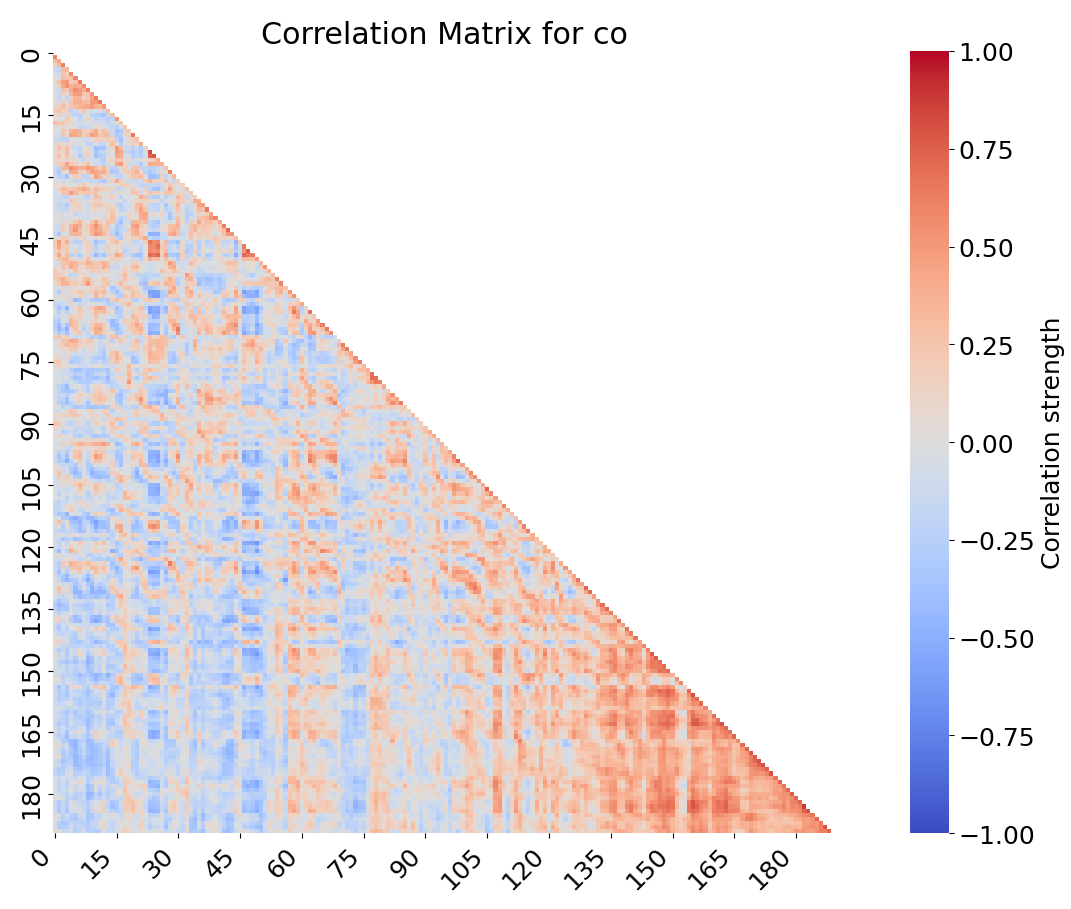
\includegraphics[width=\textwidth]{/home/nick/github_repos/Pollution-Autoencoders/paper-draft/images/corr_matrix.png}
\caption{Correlation Matrix}
\label{fig:matrix}
\end{figure}

\par As previously mentioned in the introduction, the correlation between features was revealed to be rather high. In particular, days one hundred thirty-five to one hundred-eighty nearly all have a correlation coefficient greater than 0.75. This resulted in some overfitting which can be seen in the autoencoder and pca explainable variance scores, which were greater than the unencoded scores.

\newpage
\begin{Center}
\begin{figure}[h!]
\caption{Data Pipeline}
\label{fig:pipeline}
    \hspace{1.5cm}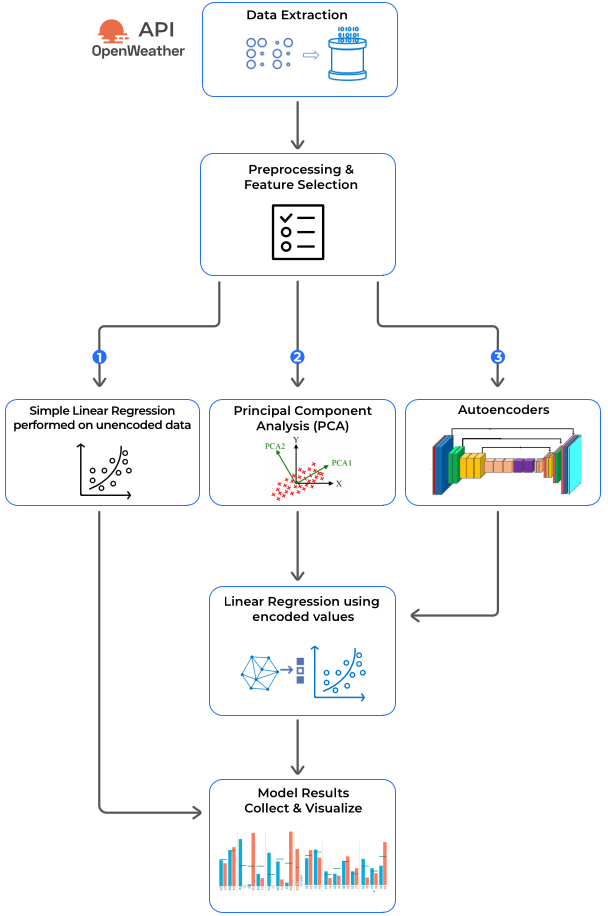
\includegraphics[width=10cm, height=13cm]{/home/nick/github_repos/Pollution-Autoencoders/paper-draft/images/pipeline.png}
\end{figure}
\end{Center}

\subsection{Data Collection and Preprocessing}
The dataset was created using OpenWeather's Air Pollution API. The dataset includes data for 
eight polluting gases and particulates: CO, NO, NO$_2$, O$_3$, SO$_2$, NH$_3$, PM$_{2.5}$, 
and PM$_{10}$. Also included was the city name, hourly timestamp, the latitude and longitude (part of the input), and the air quality index (aqi). We chose not to use the aqi because it is overall less sensitive to change and is unlikely to reveal any long-term patterns over such a short time span .
\par We looked at data for the eight pollutants over a five month time frame: January 27th, 2020 through June 6th, 2021. The final dataset includes just over eighteen thousand cities in the United States and other U.S. territories. We found it easier to focus on a single gas when developing the models, so we chose to concentrate on CO during the engineering process. The same process was then applied to the other seven gases and particulates after the development was completed.

% dataset characteristics table
\begin{table}[h!]
    \caption{Dataset Characteristics}
    \label{tab:table1}
    \vspace{0.1cm}
    \begin{tabular}{p{4cm}p{7cm}}
        \hline
        \multicolumn{2}{c}{OpenWeather Pollution API} \\
        \hline
        Sampling period  & 11/27/20 to 06/05/21\\
        Time interval & Daily  \\
        Cities & 18,526 \\
        Features & 190 \\
        Component gases & 8 \\
        Dependent variable & Last day of the period (06/05/21) \\
        \hline
    \end{tabular}
\end{table}
\par OpenWeather's Pollution API ordinarily returns hourly values, but we opted to use the daily average pollution levels as our feature set in order to make the number of starting dimensons more manageable. The daily averages were also feature engineered to be proportional to the number of features so as to avoid the curse of dimensionality \parencite{Trunk79}. 
\par The original data was unit normalized so that the gradient descents could converge more quickly while still preserving the original differences in range. Each step was saved separately to provide expeditious access to both the normalized and non-normalized data.

\subsection{Autoencoder Model}
\par The autoencoder model used consists of a single encoded and decoded layer. The data was split into a train and test set at the beginning of the testing cycle, and was further separated into a validation set for each given dimension. The validation set was essential for updating the model weights after every epoch. After the model was trained and validated, we created the finalized embeddings using the full dataset. We created embeddings for several of the most significant dimensions based off their increase in explained variance scores.

\subsubsection{Model Validation}
\par A grid search was performed for each model to determine the optimal hyperparameters. The following hyperparameters were tested:
\begin{itemize}
    \item \textit{Learning Rate:} 0.0001, 0.001, 0.01, 0.1
    \item \textit{Batch Size:} 32, 64, 128, 256
    \item \textit{Epochs:} 10, 50, 75, 100
\end{itemize}
\par K-folds cross validation was implemented to validate the grid search using five folds. Additional, the training split for each dimension was separated into a validation set. Each hyperparameter was selected based on the highest coefficient of determination that appeared in each of the five folds for every given dimension. The most frequently occuring combination of hyperparameters was then used to create the finalized embedding. The lowest coefficients of determination were saved and compared with the highest values to give an upper and lower bound of expected values.
\par After some preliminary testing, it was decided that the activation, optimizer, and loss functions should remain constant. The exponential increase in computing time this would have on the grid search drastically outweighed any minor performance gains that a thorough optimization of these functions may have yielded.

\begin{table}[h!]
    \caption{Constant hyperparameters used across all autoencoder models}
    \label{tab:table1}
    \vspace{0.1cm}
    \begin{tabular}{p{4cm}p{7cm}}
        \hline
        \multicolumn{2}{c}{Constant Hyperparameters}\\
        \hline
        Activation function & tanh\\
        Loss function & Mean Squared Error  \\
        Optimizer & Adam \\
        \hline
    \end{tabular}
\end{table}
Moreover, grid search was only performed on a select number of key dimensions rather than on all one hundred ninety dimensions. The first ten dimensions, as well as every tenth dimension until one hundred-twenty were tuned. For each intermediary dimension that did not have a set of key hyperparameters, the hyperparameters of the previous key dimension was used. Once again, the tradeoff between minor performance gains and large compute times led us to adjust the scope of the  hyperparameter tuning.

\begin{table}[h!]
    \caption{Grid Search Results for Carbon Monoxide}
    \label{tab:table2}
    \vspace{0.1cm}
    \begin{tabular}{p{2cm}p{2cm}p{2cm}p{2cm}p{2cm}}
        \hline
        \multicolumn{5}{c}{CO Grid Search Key Dimensions 1-10}\\
        \hline
        dimension & $r^{2}$ & learning rate & batch & epochs  \\
        1 & 0.22 & 0.01 & 64 & 10 \\
        2 & 0.44 & 0.0001 & 256 & 50\\
        3 & 0.49 & 0.001 & 64 & 50\\
        4 & 0.52 & 0.0001 & 32 & 50\\
        5 & 0.56 & 0.0001 & 32 & 100\\
        6 & 0.57 & 0.01 & 32 & 10\\
        7 & 0.60 & 0.0001 & 32 & 150\\
        8 & 0.63 & 0.0001 & 64 & 150\\
        9 & 0.62 & 0.0001 & 32 & 150\\
        10 & 0.62 & 0.0001 & 64 & 100\\
        \hline
    \end{tabular}
\end{table}
\begin{table}[h!]
    \caption{Grid Search Results for Carbon Monoxide}
    \label{tab:table2}
    \vspace{0.1cm}
    \begin{tabular}{p{2cm}p{2cm}p{2cm}p{2cm}p{2cm}}
        \hline
        \multicolumn{5}{c}{CO Grid Search Key Dimensions 20-120}\\
        \hline
        dimension & $r^{2}$ & learning rate & batch & epochs  \\
        20 & 0.62 & 0.01 & 64 & 50\\
        30 & 0.64 & 0.01 & 128 & 75\\
        40 & 0.67 & 0.01 & 256 & 100\\
        50 & 0.68 & 0.01 & 64 & 75\\
        60 & 0.69 & 0.001 & 32 & 150\\
        70 & 0.70 & 0.001 & 64 & 150\\
        80 & 0.71 & 0.001 & 32 & 150\\
        90 & 0.71 & 0.01 & 64 & 100\\
        100 & 0.72 & 0.01 & 64 & 150\\
        110 & 0.72 & 0.01 & 32 & 75\\
        120 & 0.73 & 0.001 & 64 & 100\\
        \hline
    \end{tabular}
\end{table}
\newpage

\subsection{Principle Component Analysis}
The PCA model was trained with k-fold cross-validation using five folds. The dataset was split into a training and test set. The trained PCA models were used to create embeddings at different scales of dimensionality based on the number of input components. We prioritized the first ten dimensions because they generally represent the largest increase in the percent explained variance.

\subsection{Additional Model Validation}
In addition to the PCA and Autoencoder models, a linear regression was performed on the unencoded features. The resulting explainable variance scores serve as a benchmark with which we can compare each model's data loss. 

\begin{figure}[h!]
    \centering
    \caption{Unencoded R2 Scores}
    \label{fig:pipeline}
    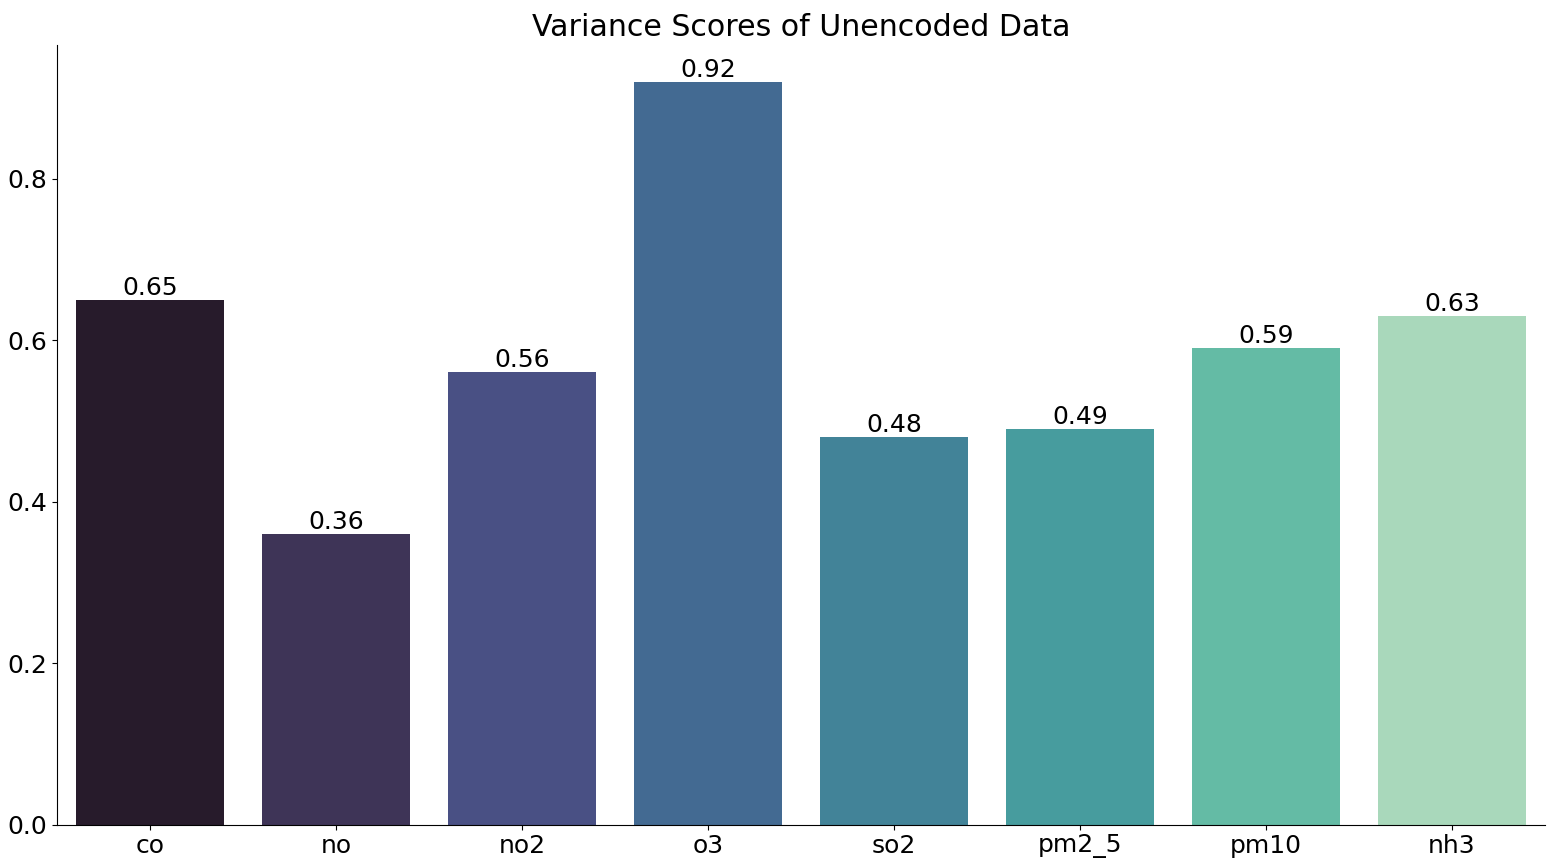
\includegraphics[width=0.8\linewidth]{/home/nick/github_repos/Pollution-Autoencoders/paper-draft/images/unencoded_r2.png}
\end{figure}

\section{Results}
We compared the percent explained variance across one hundred ninety dimensions for the encoded values generated by the PCA and autoencoder models. While PCA was overall less noisy, we found that the autoencoder model achieved a much higher explainable variance for the first several dimensions.
\comment{
\\ \note{Note that results graphs are placeholders}
% ae vs pca linegraph

\begin{figure}[h!]
\begin{subfigure}{0.5\textwidth}
    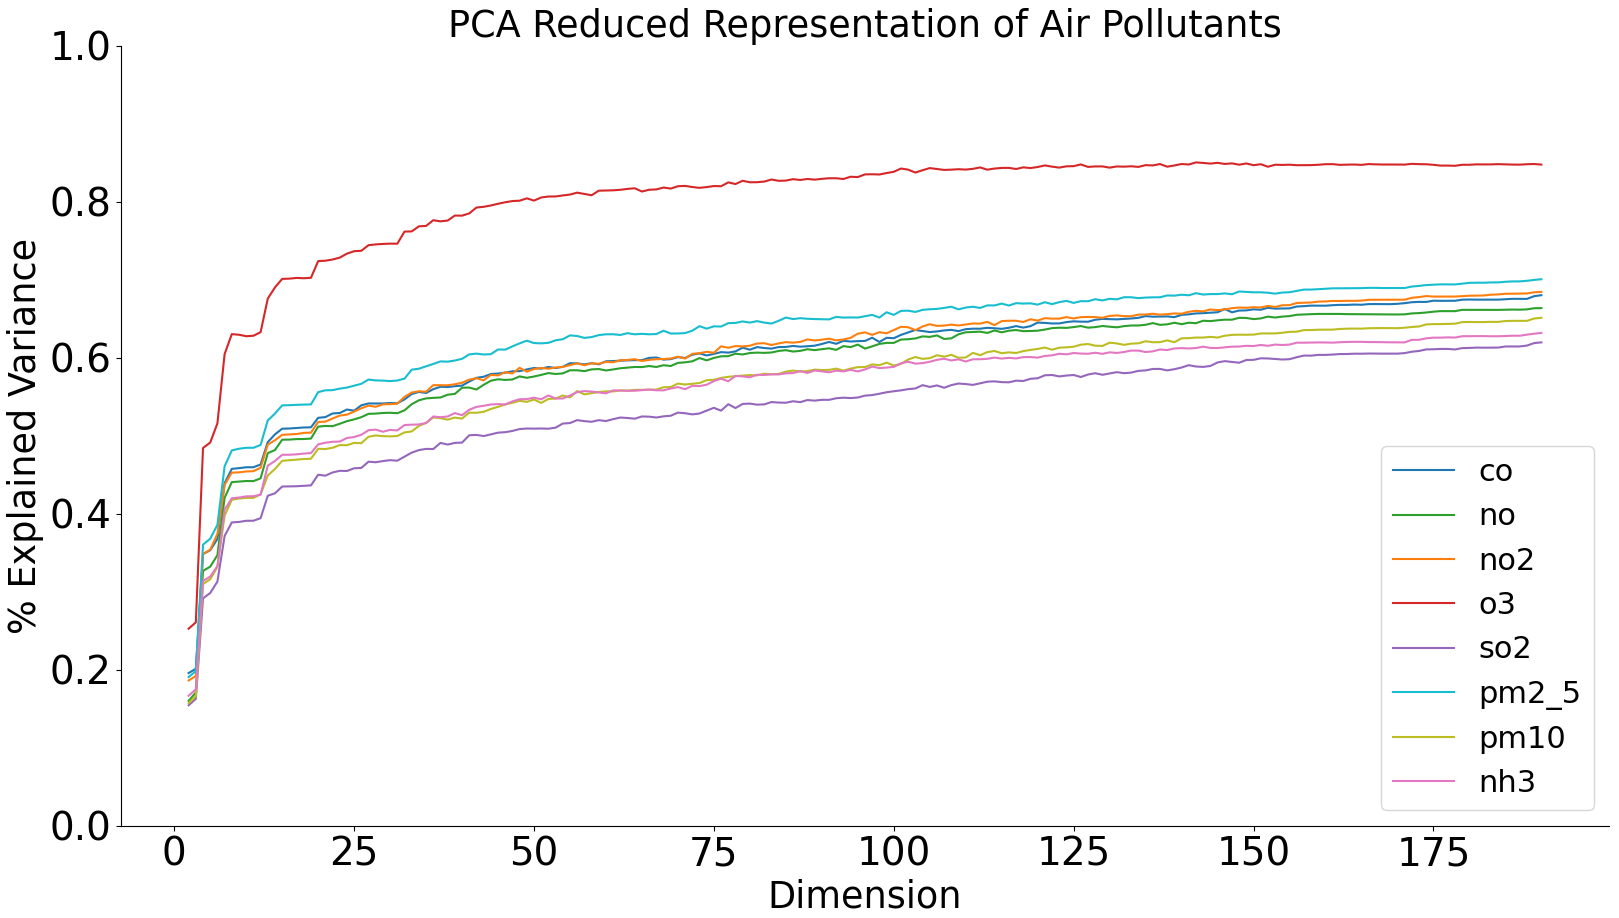
\includegraphics[width=1.1\linewidth, height=4cm]{/home/nick/github_repos/Pollution-Autoencoders/paper-draft/images/pca_all_dims.png} 
    \caption{PCA Dimensionality Reduction}
    \label{fig:ae_dim_reduction}
\end{subfigure}% <- % sign must be here!
\begin{subfigure}{0.5\textwidth}
    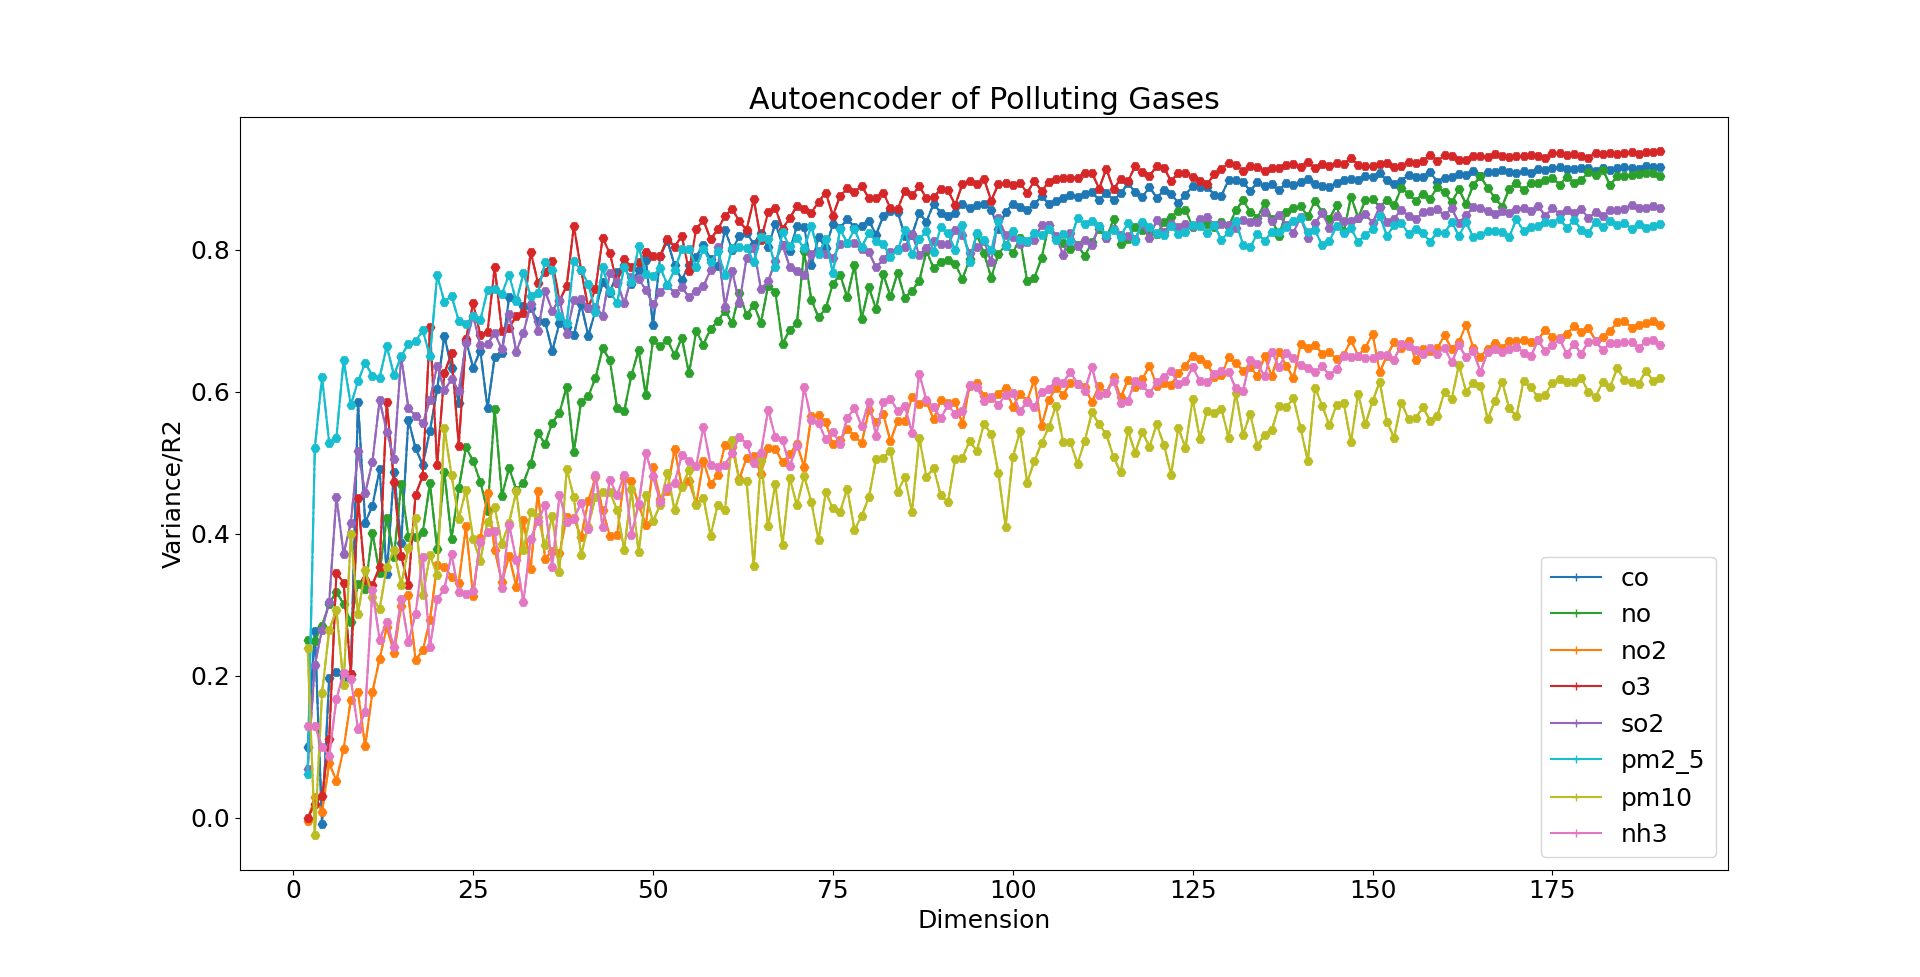
\includegraphics[width=1.1\linewidth, height=4cm]{/home/nick/github_repos/Pollution-Autoencoders/paper-draft/images/ae_all_dims.png}
    \caption{PCA Dimensionality Reduction}
    \label{fig:pca_dim_reduction}
\end{subfigure}
\caption{Graph of autoencoder and PCA reduced representations of air pollutants}
\label{fig:ae_vs_pca}
\end{figure}
}

\begin{figure}[h!]
    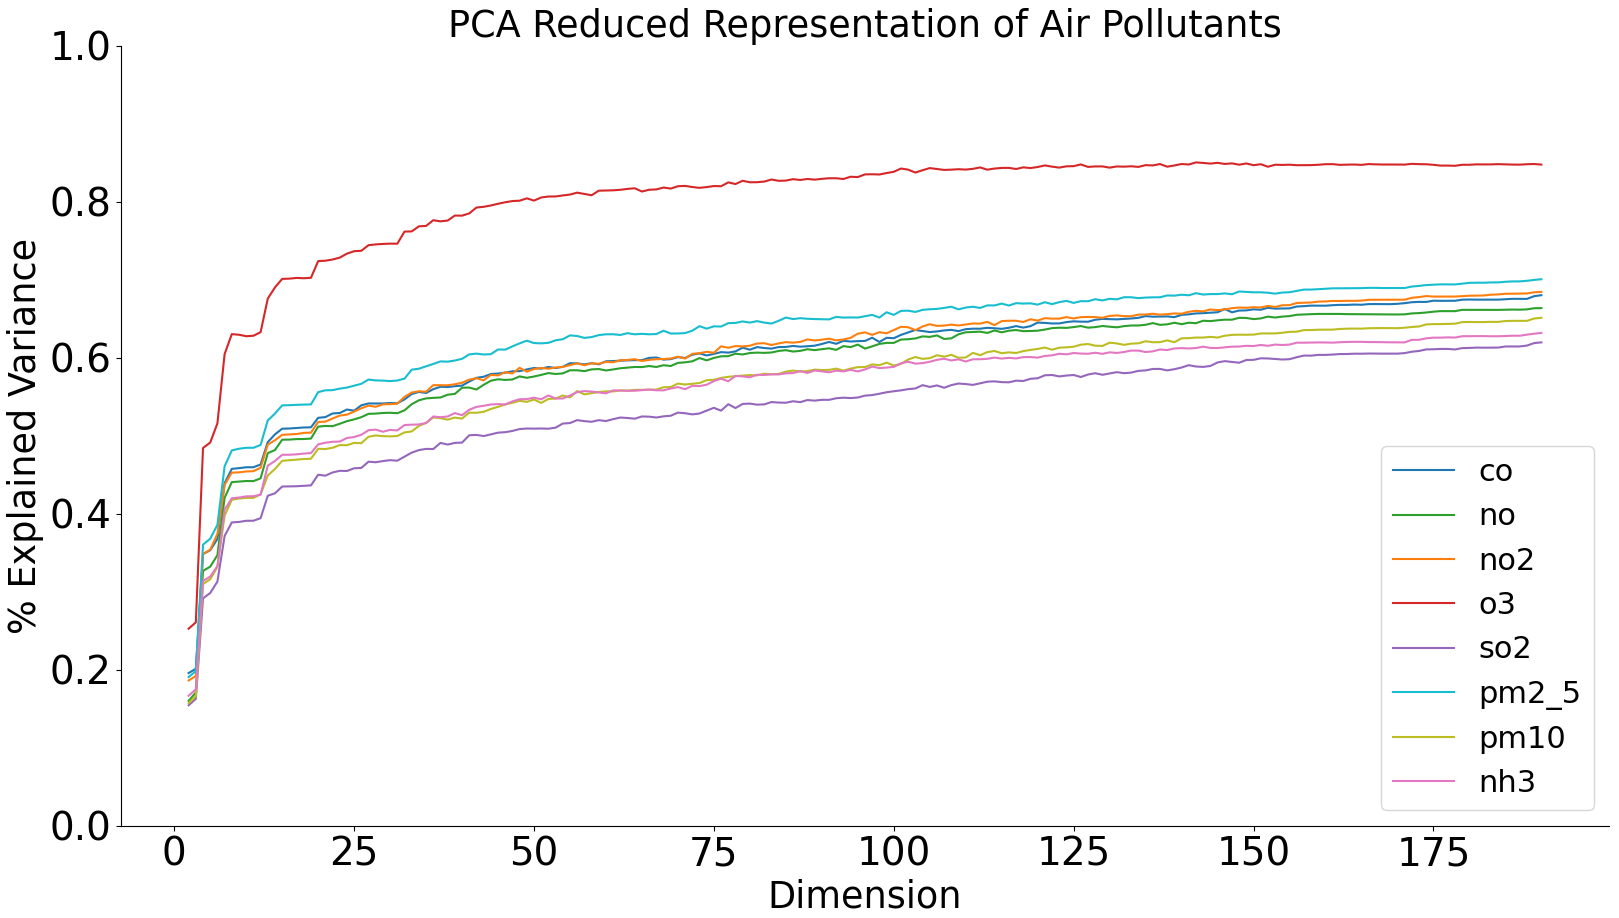
\includegraphics[width=\textwidth]{/home/nick/github_repos/Pollution-Autoencoders/paper-draft/images/pca_all_dims.png} 
    \caption{PCA Dimensionality Reduction}
    \label{fig:ae_dim_reduction}
\end{figure}

\begin{figure}[h!]
    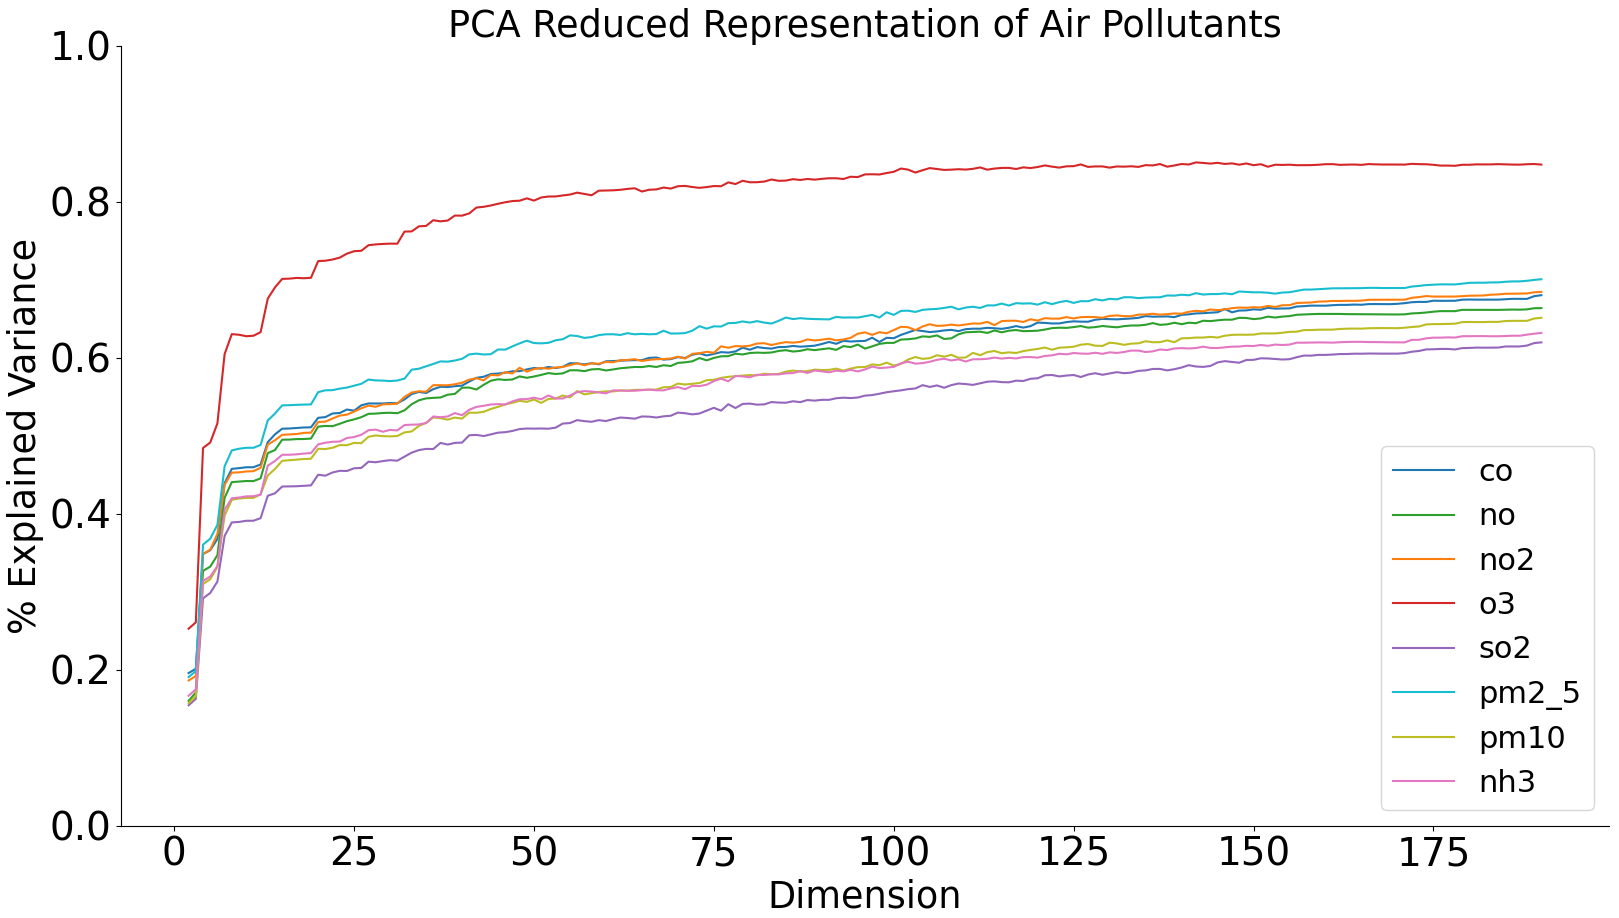
\includegraphics[width=\textwidth]{/home/nick/github_repos/Pollution-Autoencoders/paper-draft/images/pca_all_dims.png} 
    \caption{Autoencoder Dimensionality Reduction\ \note{Placeholder for AE}}

    \label{fig:ae_dim_reduction}
\end{figure}

\par We clustered the cities based on the first two latent dimensions in order to see how
the model characterizes each city

% co scatter
\begin{figure}[h!]
\begin{subfigure}{0.5\textwidth}
    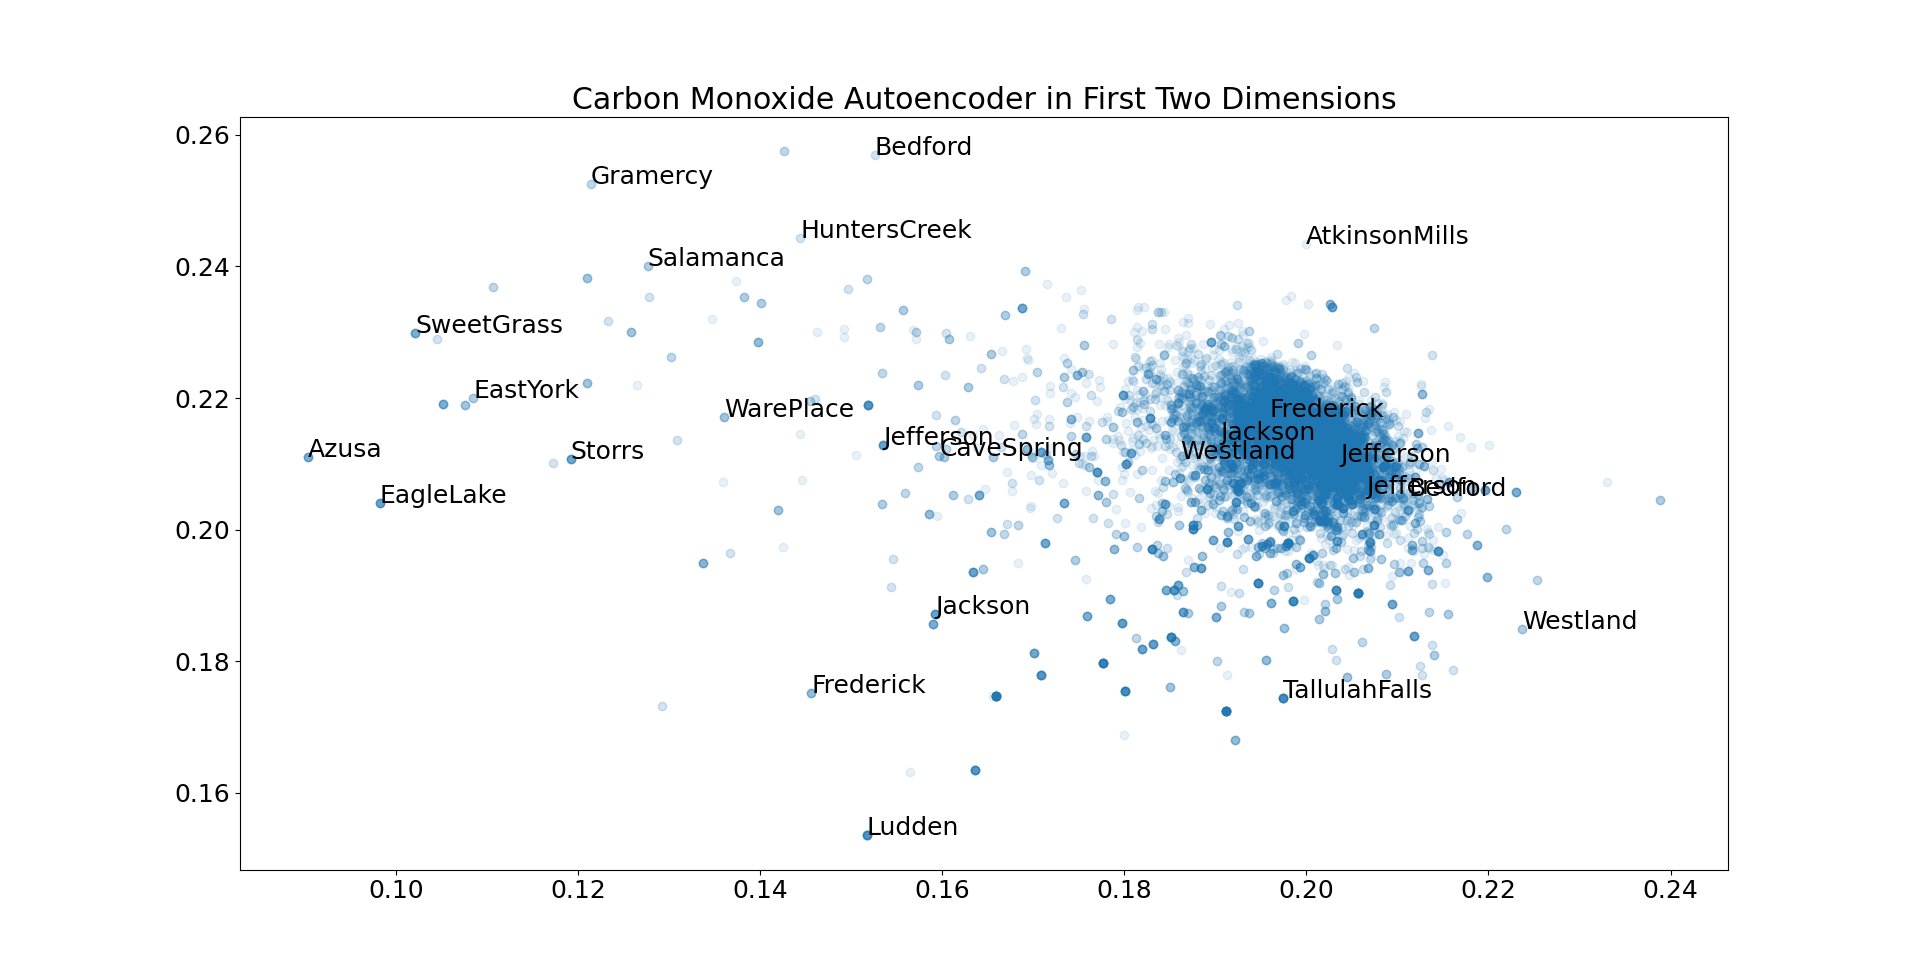
\includegraphics[width=1.1\linewidth, height=5cm]{/home/nick/github_repos/Pollution-Autoencoders/paper-draft/images/co_scatter_ae_wlist.png} 
    \caption{Outlier Cities}
    \label{fig:outliers}
\end{subfigure}% <- % sign must be here!
\begin{subfigure}{0.5\textwidth}
    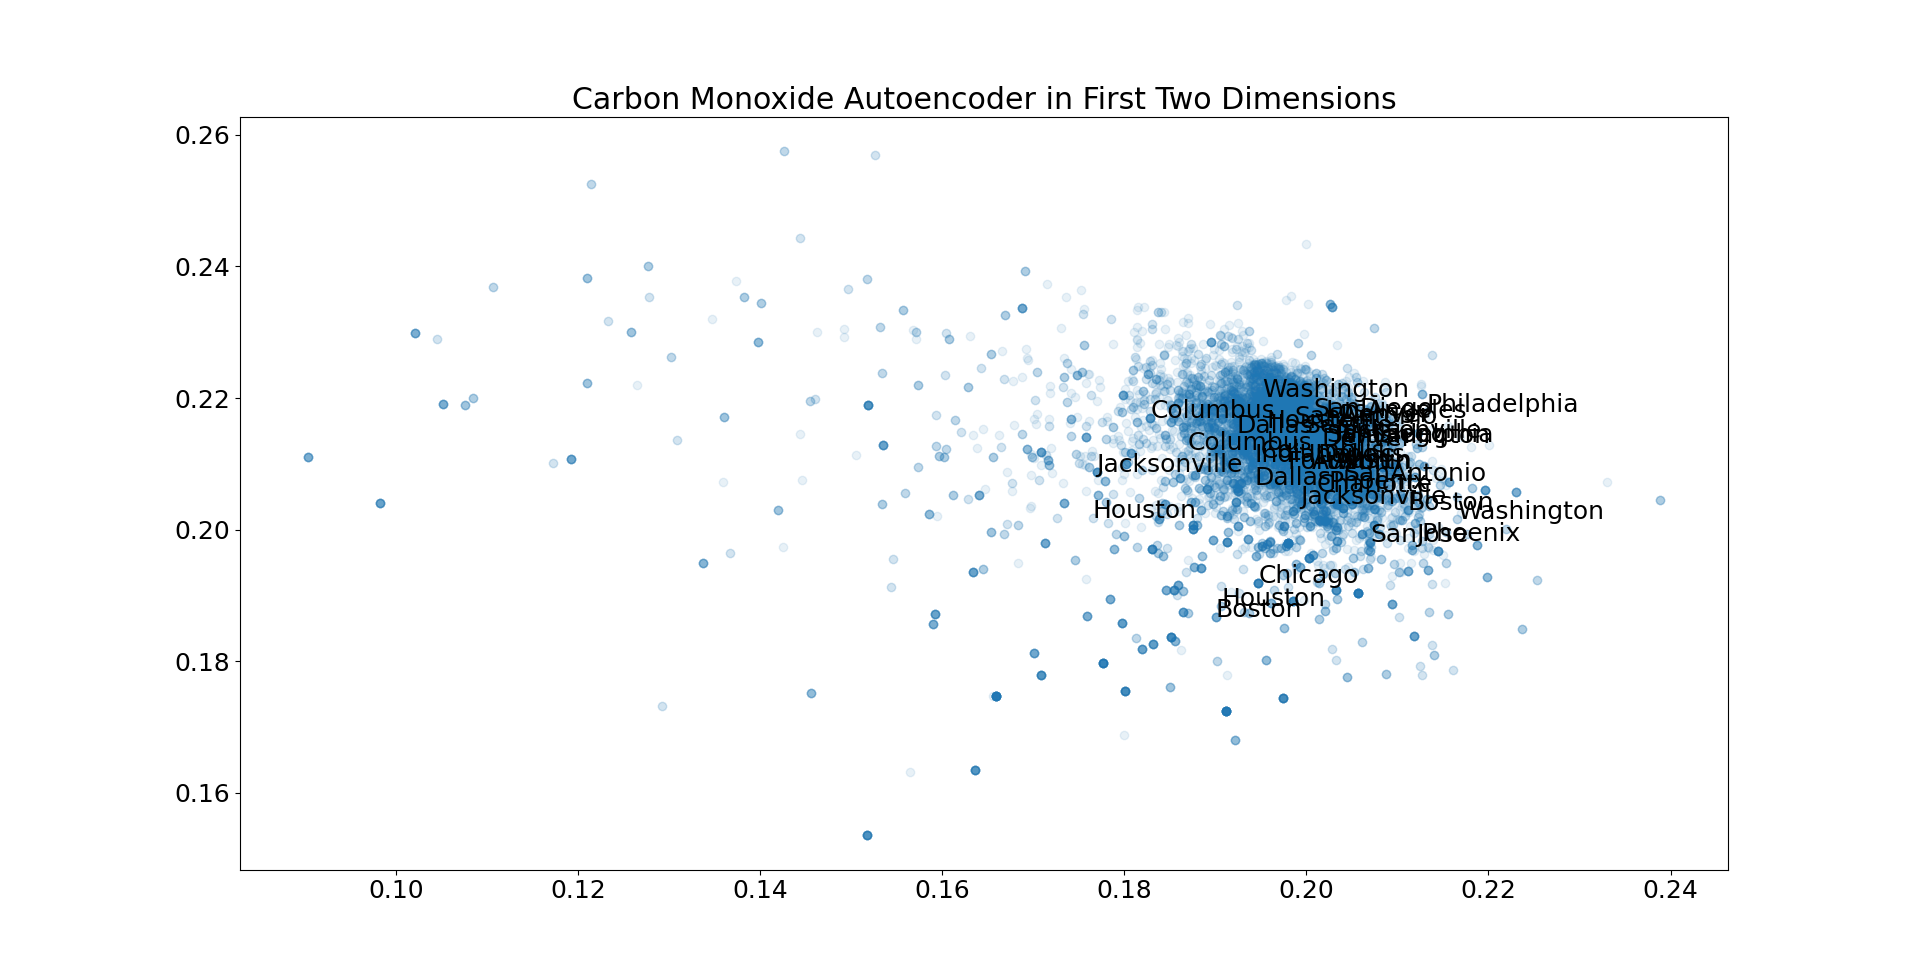
\includegraphics[width=1.1\linewidth, height=5cm]{/home/nick/github_repos/Pollution-Autoencoders/paper-draft/images/co_scatter_ae_large_cities.png}
    \caption{Densely Populated Cities}
    \label{fig:dense_cities}
\end{subfigure}

\caption{Scatter plots of outlier and highly-populated cities over first two dimensions}
\label{fig:outliers_vs_dense_cities}
\end{figure}

\par By selecting from a list the top two hundred most highly-populated cities in the US, we found that nearly all of them were located near the center of the clustering. Conversely, we found that many of the outliers were smaller cities in rural locations. 

\section{Discussion}

\section{Conclusion}

\printbibliography

\end{document}
